\documentclass[11pt]{article}
\usepackage{acl2014}
\usepackage{times}
\usepackage{url}
\usepackage{latexsym}
\usepackage{color}
\usepackage{graphicx}
\newcommand{\eat}[1]{\ignorespaces}

\newcommand{\ddcomment}[1]{\textcolor{red}{[$^{\textsc{D}}_{\textsc{D}}$ #1]}}
\newcommand{\spcomment}[1]{\textcolor{blue}{[$^{\textsc{S}}_{\textsc{P}}$ #1]}}
\newcommand{\jmcomment}[1]{\textcolor{magenta}{[$^{\textsc{J}}_{\textsc{M}}$ #1]}}

\setlength\titlebox{6.5cm}    % Expanding the titlebox

\title{Enhanced Search with Wildcards and Morphological Inflections\\in the Google Books Ngram Viewer}

\eat{\author{Jason Mann, David Zhang, Lucille Yang, Slav Petrov and Dipanjan Das\\
	Google Inc. \\
	{\tt jcm2207@columbia.edu, dzhang21@gmail.com, ly77@cornell.edu}\\
	{\tt \{slav,dipanjand\}@google.com}}
}

\date{}

\begin{document}
\maketitle

\begin{abstract}

We present a new version of the Google Books Ngram Viewer, which plots
the frequency of words and phrases over the last five
centuries; its data encompasses 6\% of the world's published books.
The new Viewer adds three features for more powerful search: wildcards,
morphological inflections, and case insensitivity. These additions allow
the discovery of patterns that were previously difficult to find in the Google Books Ngram data,
and further facilitate the study of linguistic trends in printed text.

\end{abstract}

\section{Introduction}

The Google Books Ngram Viewer\footnote{See \url{http://books.google.com/ngrams}.} and its associated Google Books Ngram Corpus \cite{lin2012syntactic} are useful tools for the analysis of cultural, social and linguistic trends through five centuries of written text in eight languages. To cite a few examples, they have been used to detect emotion trends in 20th century books \cite{acerbi.etal.2013}, to analyze text focusing on market capitalism throughout the past century \cite{Schulz2013}, detect social and cultural impact of personalities throughout history \cite{skiena.ward.2013}, or analyzing the correlation of economic crises with a literary `misery index' reflected in printed text during crises
periods \cite{bentley.et.al.2014}.

In this paper, we present an updated version of the Viewer which introduces several new features, enabling
used to issue more interesting and powerful search queries. First, users can replace one query term with a placeholder symbol (wildcard, henceforth), which will return the ten most frequent replacements in the underlying corpus for the specified year range. Second, by adding a specific tag to any word in a query, morphological inflections (or variants) will be returned. Finally, the new interface has a new option to allow for multiple capitalization styles. Figure~\ref{fig:examples} provides examples for these three new types of queries.
In addition, this demonstration presents an overhaul of the Viewer's user interface, with interactive features that allow for easier management of the increase in data points returned.

\begin{figure*}
\centering
\hspace*{-0.5cm}
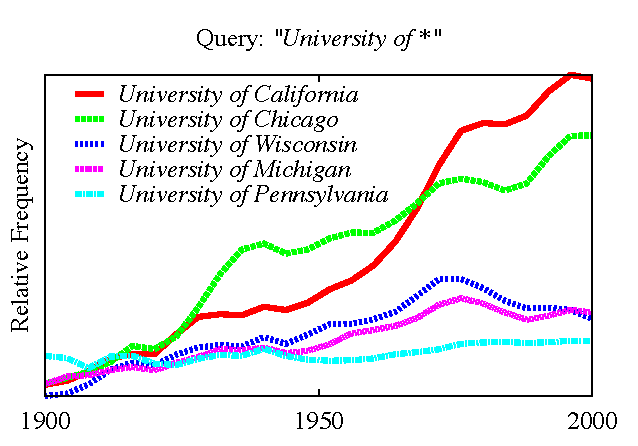
\includegraphics[width=0.33\textwidth]{graphs/university}
\hspace*{0.1cm}
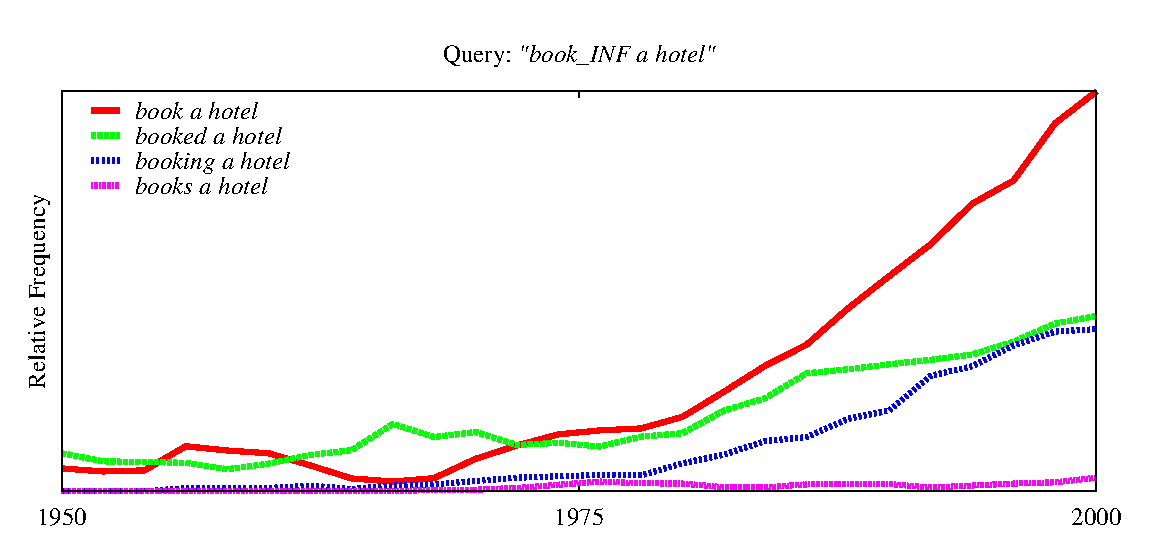
\includegraphics[width=0.33\textwidth]{graphs/book}
\hspace*{0.1cm}
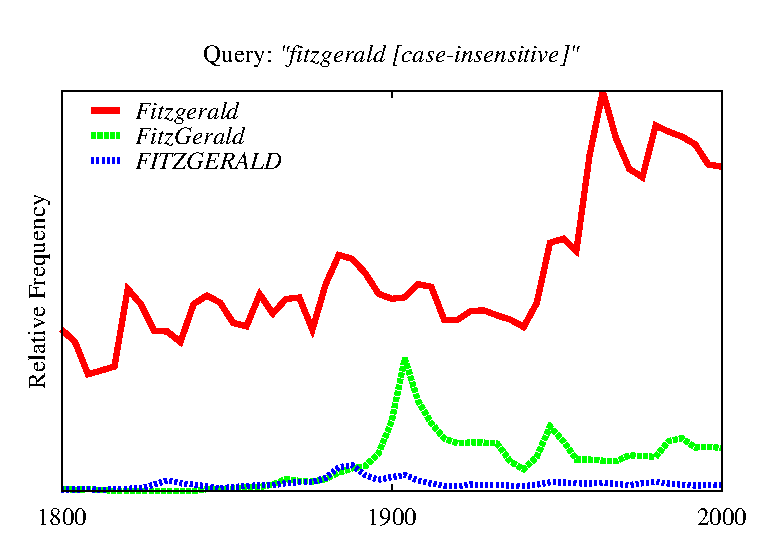
\includegraphics[width=0.33\textwidth]{graphs/fitzgerald}
\hspace*{-0.5cm}
\vspace*{-0.25cm}\caption{\label{fig:examples}
Example queries highlighting the new functionality. Figures need to be updated. Just a placeholder for now.}
\end{figure*}

While it is obvious how the above searches can be answered via brute-force computation, supporting an interactive application with low latency necessitates some precomputation. To this end, we provide an overview of our system architecture in \S\ref{sec:overview} and discuss some of our design choices. We then detail interesting use cases in \S\ref{sec:usecases}, which were difficult (or even impossible) to search in the previous versions of the Ngram Viewer that did not handle wildcards in the search queries. Additionally, we detail how the two other aforementioned features introduced in this demonstration paper result in interesting retrieval results. Beyond specific search queries, we envision the new functionality of the tool uncovering trends and patterns not readily apparent in the data.

\section{System Overview}
\label{sec:overview}

In this section we present an overview of the system architecture. We briefly review the underlying corpus and architecture of previous versions of the Viewer \cite{culturomics,lin2012syntactic} and then focus on the extensions added in this version. It should be emphasized that this demonstration updates only the Viewer, and provides tools for easier analysis of the underlying data. The ngram data itself is not updated and is identical to that of \newcite{lin2012syntactic}.


\subsection{Ngram Corpus}
	The Google Books Ngram Corpus\footnote{Downloadable from \texttt{https://books.google.com/} \texttt{ngrams/datasets}.} provides ngram counts for eight different languages over more than 500 years; additionally, the English corpus is split further into British vs. American English and Fiction to aid domain restriction. This corpus is a subset of all the books digitized at Google, and represents more than 6\% of all publicized texts in its newest edition \cite{lin2012syntactic}. The differences between the first and second versions of the corpus are discussed at length in the aforementioned paper.
	

Sentences from the Google Books Corpus are tokenized and segmented based on manually devised rules\footnote{Excluding Chinese, where a statistical segmentation system is used} that also capture those that span across page boundaries. \textsf{\textsc{\_start\_}} and \textsf{\textsc{\_end\_}} designate beginning and end tokens for distinguishing sentence medial ngrams from those near sentence boundaries \cite{lin2012syntactic}.

The current version of the corpus is tagged using the universal part-of-speech tag set containing twelve coarse categories, as described by \newcite{petrov2012universal}. Individual words exist in both tagged and untagged forms for all ngrams up to a length of three, including dependency relations. The dependency ngrams are created according to \newcite{lin2012syntactic} and specify pairwise syntactic relationships between words in the same sentence. These relationships are shown by directed arcs that specify a single head word for each sentence. Also, in raw ngrams of up to length three, POS tags can stand in place of a word to represent the sum of all the ngram counts for that specific tag. When combined with the tools we describe below, these tags provide a further layer of abstraction in a query.



\subsection{Architecture}
The Viewer provides a lightweight interface to the underlying ngram corpora. In its basic form, user requests are directed through the server to a simple lookup table containing the raw ngrams and their frequencies. This data flow is displayed in the top part of Figure \ref{fig:architecture} and is maintained for queries containing none of the tools offered by the update.

The new types of queries could be in principle be implemented by scanning the raw ngrams on the fly and returning the relevant subset. Given the large quantity of ngrams, such an approach would be computationally very expensive and too slow for an interactive application. We therefore pre-compute intermediate results that can be used to more efficiently retrieve the results for the new queries. The intermediate results are stored in additional lookup tables (shown at the bottom in Figure \ref{fig:architecture}) that are queried first and then trigger potentially multiple requests to the raw ngram tables. For example, the intermediate results table for the morphological variants search contains inflected forms for all unigrams. These inflected forms are substituted for the selected query term and the resulting ngram is looked up in the raw ngram table. We describe the intermediate results tables and how they are generated in the next section.

It should be noted that we only support one expansion per query ngram. This is needed in order to avoid the combinatorial explosion that would result from mixing multiple expansions in the same ngram.



\begin{figure}
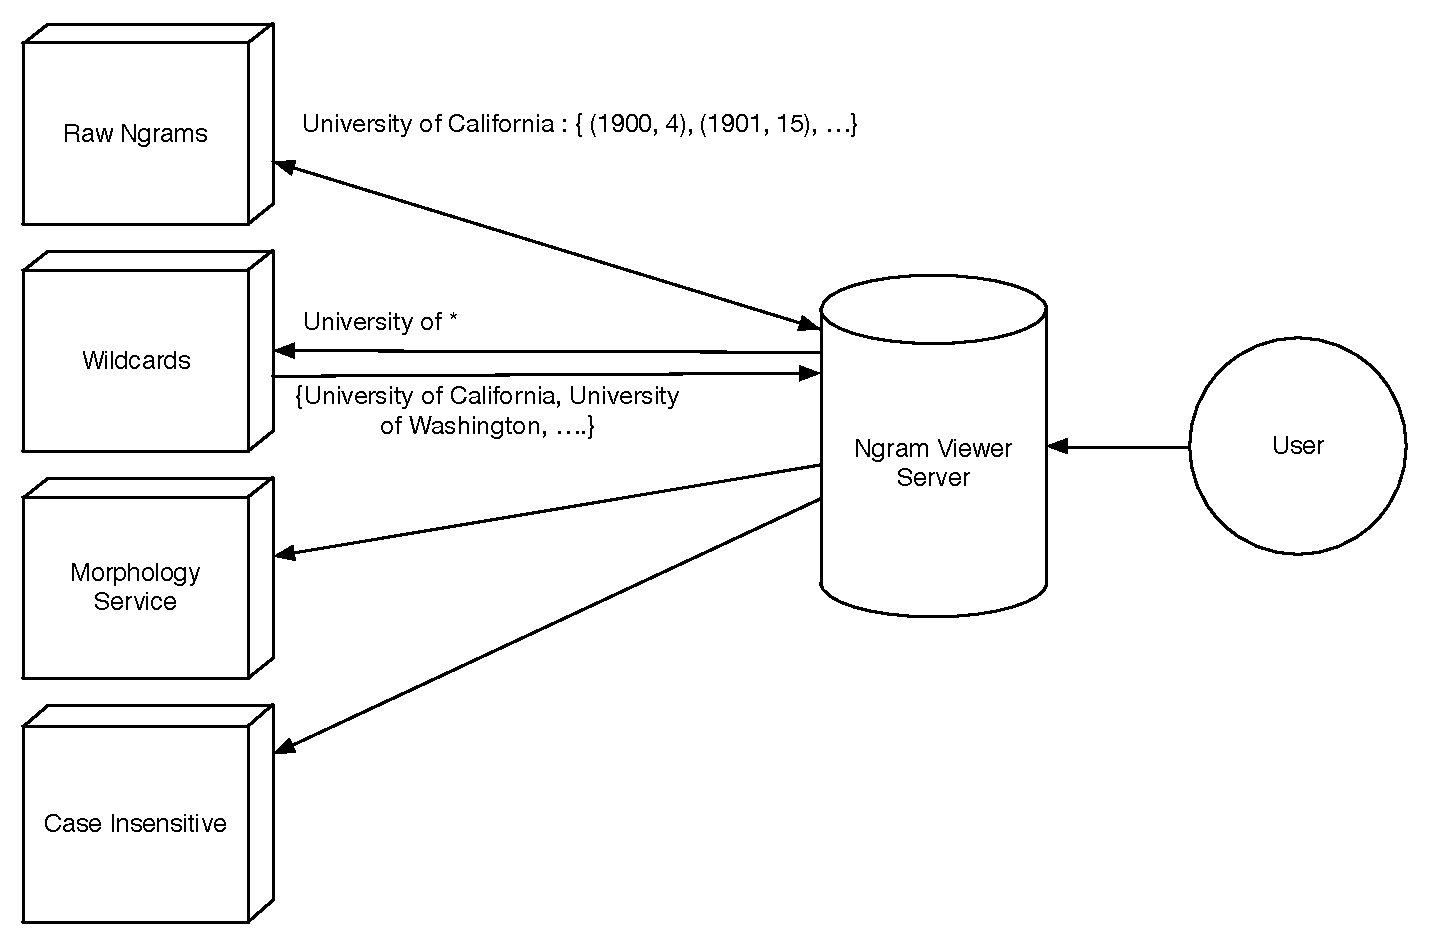
\includegraphics[width=20em,keepaspectratio=true]{system_architecture}
\caption{\label{fig:architecture}Diagram of new system architecture.}
\end{figure}


\section{New Features}
Here, we describe the novel aspects of the Ngram Viewer introduced in this demonstration paper.
\begin{table*}
\centering
\begin{tabular}{|c|c|}
\hline
\textbf{Query}	& \textbf{Possible Replacements}	\\ \hline
a * man					& a young man, a good man, a kind man, a wild man		\\ \hline
booked\texttt{=>}*\textsf{\textsc{\_noun}}	& \begin{tabular}[c]{@{}c@{}}booked\texttt{=>}flight\textsf{\textsc{\_noun}}, booked\texttt{=>}passage\textsf{\textsc{\_noun}},
						\\ booked\texttt{=>}room\textsf{\textsc{\_noun}}, booked\texttt{=>}eat\textsf{\textsc{\_noun}}\end{tabular} \\ \hline
John said\textsf{\textsc{\_inf}}			& John says, John said, John say, John saying                                                                                                                                   \\ \hline
book\textsf{\textsc{\_inf}}\textsf{\textsc{\_noun}}			& book, books                                                                                                                                                                   \\ \hline
\begin{tabular}[c]{@{}c@{}}the cook\\ (case insensitive)\end{tabular} & THE COOK, the cook, The Cook, the Cook, The cook                                                                                                                              \\ \hline
\end{tabular}
\caption{\label{tab:wildcard}
Examples of precompiled wildcard, inflection, and case insensitive queries.}
\end{table*}


\subsection{Wildcards}
\label{sec:wildcards}
	We support the use of wildcards by utilizing an additional database that stores the most frequent replacements of queries to the ngram corpus. This wildcard database is created as a pre-compilation step when creating the Ngram Corpus from the Google Books data. When a new ngram is created, one word or tag at a time is replaced with the wildcard symbol, `*', creating a wildcard query. The query becomes a key in a string indexed lookup table, and the original ngram is added to a list of ngrams which are its values. As mentioned above, due to space considerations we were not able to store all possible replacements for every wildcard ngram we precomputed. Also, we could not precompute a perfect set of the top 10 ngrams for every possible year range, while this would require intermediate storage space on the order discussed above, as well as the computation time to calculate the top 10 for $\frac{n(n+1)}{2}$ time periods for each wildcard. Instead we estimate the top 10 during the creation of wildcard ngrams, by limiting the number of replacements to the top ten for every year. We gather these top 10 lists into a union and map the raw ngrams to the wildcard ngram string in our table. 
	
	During this process, we filter punctuation from consideration as a valid replacement because in practice punctuation returns uninteresting results. On this note, it may be useful to specify a specific POS tag (i.e. `*\textsf{\textsc{\_noun}}') to provide more specific results. At runtime, union of replacement ngrams is processed for the specific year range requested and the top ten results are returned. For examples of expansions see Table \ref{tab:wildcard}. 


\subsection{Morphological Inflections}
Inflections of words in search queries are handled using a Google Search interface that can provide morphological variations of words for different syntactic categories \cite{durrett2013supervised}. As this type of request utilizes an internal API, the results from a specific request are subject to change. Unlike wildcard substitutions, there is no need for pre-computation; given a query with the keyword \textsf{\textsc{\_inf}} attached to a word (e.g., `John said\textsf{\textsc{\_inf}}'), we get the counts of all the ngrams that start with `John' and have the morphological inflections of the root form `say' as its second word in the Ngram Corpus. We have noticed that there can be more than 10 results returned per query, especially for morphologically rich languages like Russian, unlike the wildcard search feature. Therefore we have updated the user interface to better deal with more data lines (\S\ref{sec:userint}). We do not allow the combination of morphological inflections with wildcards and/or case insensitive searches
because it slows down the retrieval process.

\subsection{Case Insensitive}
Case insensitive searches are enabled by selecting a check box on the new interface. These queries, like the wildcards, are referenced to a separate database that contains a mapping of different case combinations to the ngram string in lowercase. The possible combinations of case are: ALL CAPS, first letter Capitalization (all possible variations), and all lower case. During experimentation, we noticed that often there are many case variants of a given query for which the ngram counts are negligible; hence, to keep our retrieved results meaningful, we filter out all case variants that have a cumulative count of less than 1\% of the most frequent case variant for a given year range.



\subsection{User Interface}
\label{sec:userint}
Due to the increased number of results returned per query, we have also updated the user interface. Interactive functionality allows the user to highlight a line by hovering over it, keep that focus by left clicking, and clear all focused lines by double clicking. For any of the three queries mentioned above, you may also right click on any of the queries returned to combine them into the total line for the wildcard query. Another feature added to the interface is static URLs which maintain all of the raw ngrams retrieved from any query. This is to prevent statically linked charts from changing over time, and allowing for backwards compatibility.


\section{Use Cases}
\label{sec:usecases}
We present multiple use cases that can be captured using the several features that we have presented in this paper. First, we show some examples of each of these individual features; next, we present some example queries that combine queries that use syntactic annotations and the current additions to exhibit the type of results that the Ngram Viewer can retrieve.

\subsection{Base Wildcards vs. Specified POS}
We have found that searches using the base wildcard '*' often return unsatisfying results. It is often more beneficial to include the desired POS tag in combination with the wildcard search (i.e. `*\textsf{\textsc{\_noun}}')

\jmcomment{Most popular words for context across year ranges or languages}
\begin{figure*}
\centering
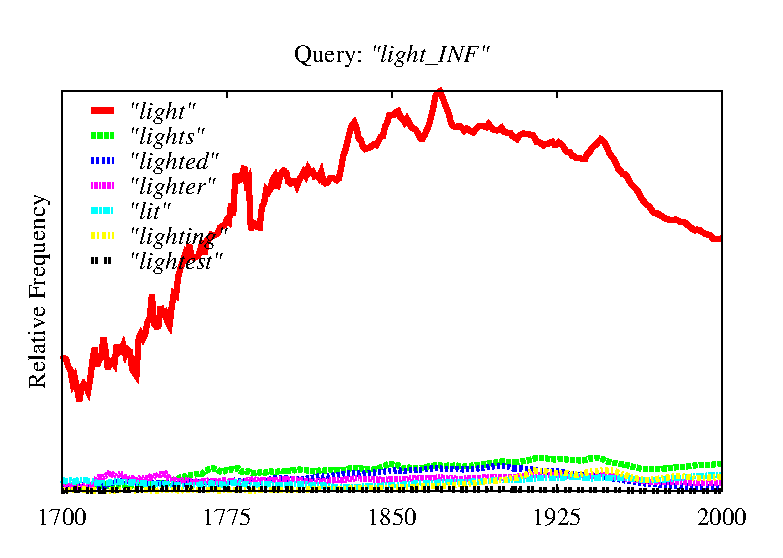
\includegraphics[width=.48\textwidth]{graphs/light_INF}
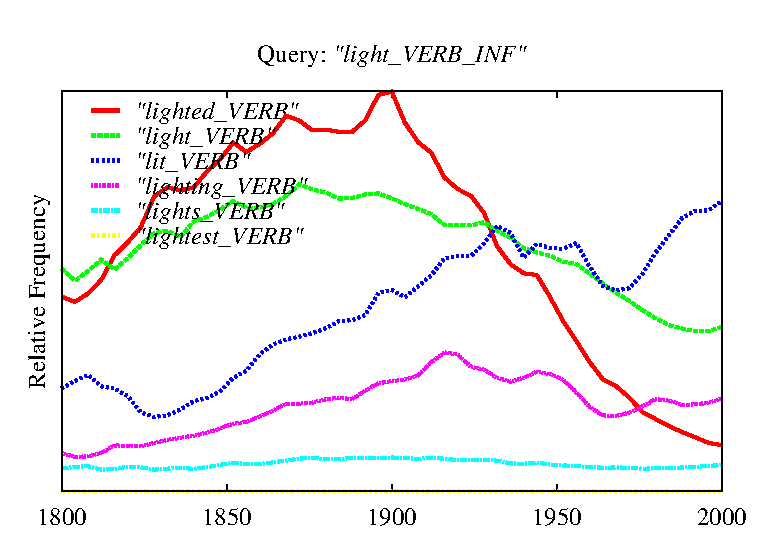
\includegraphics[width=.48\textwidth]{graphs/light_INF_VERB}
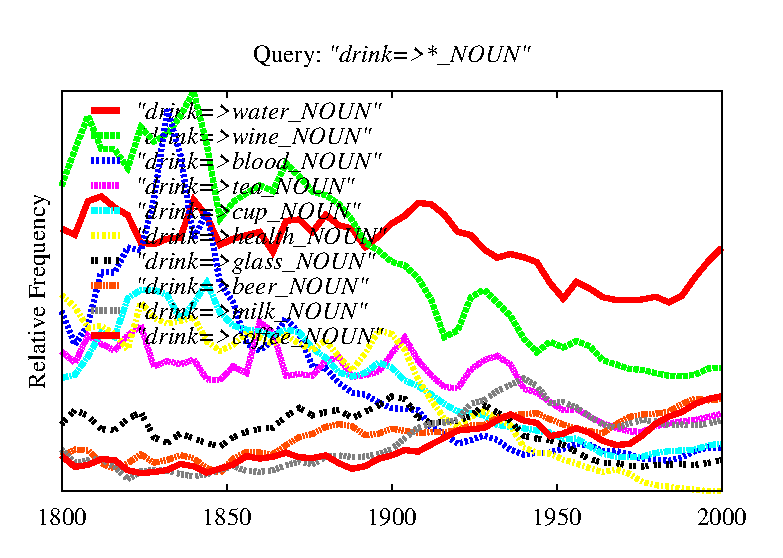
\includegraphics[width=.48\textwidth]{graphs/drink}
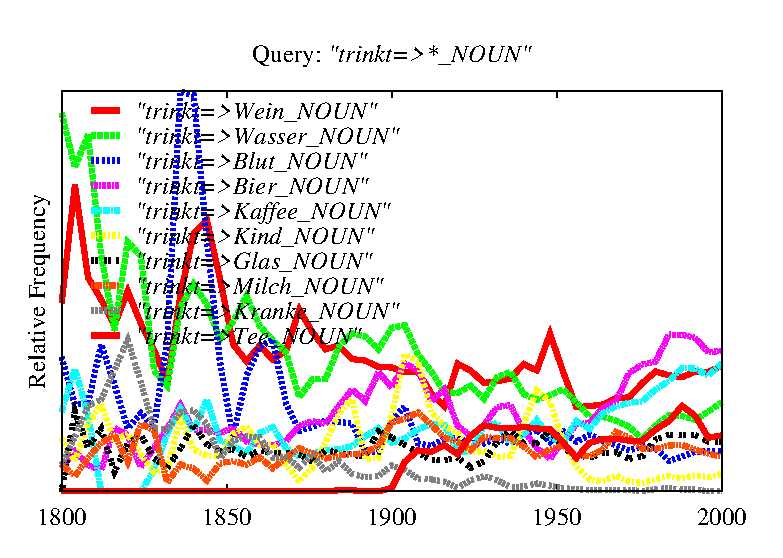
\includegraphics[width=.48\textwidth]{graphs/drink_GER}
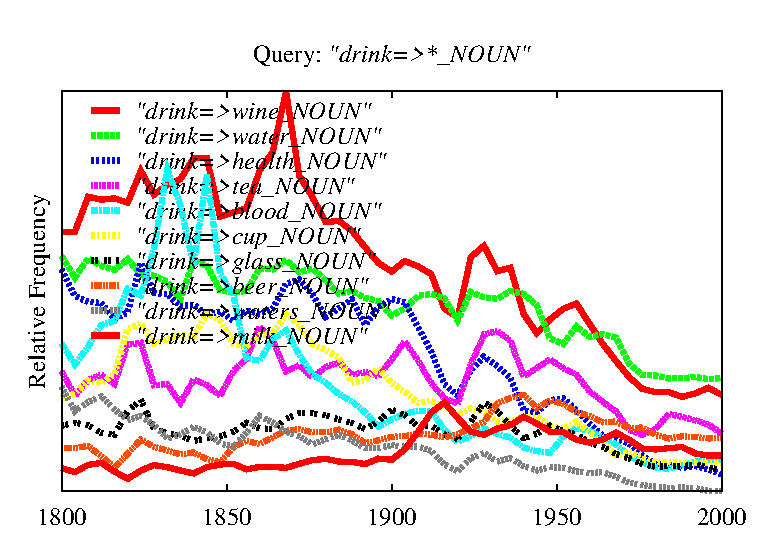
\includegraphics[width=.48\textwidth]{graphs/drink_UK}
\eat{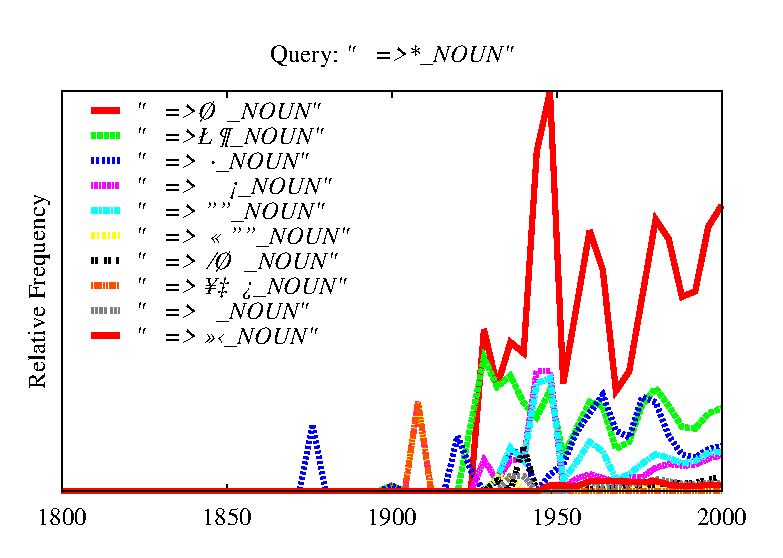
\includegraphics[width=.48\textwidth]{graphs/drink_CHI}
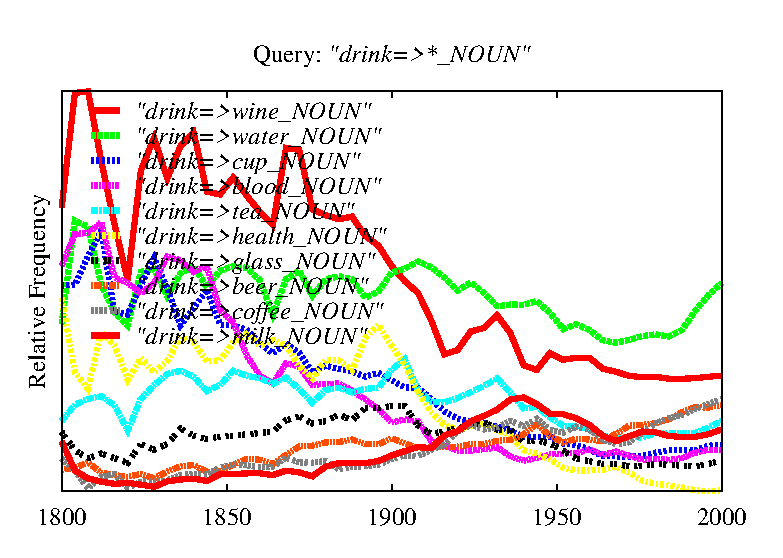
\includegraphics[width=.48\textwidth]{graphs/drink_USA}
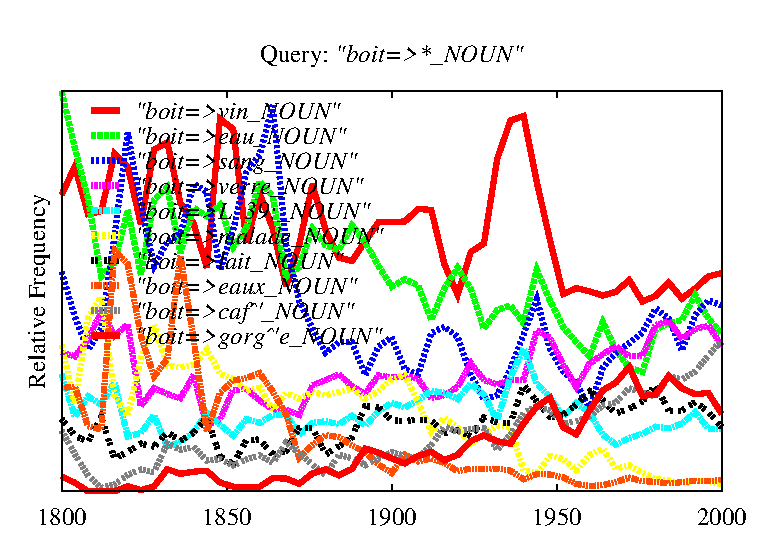
\includegraphics[width=.48\textwidth]{graphs/drink_FRE}
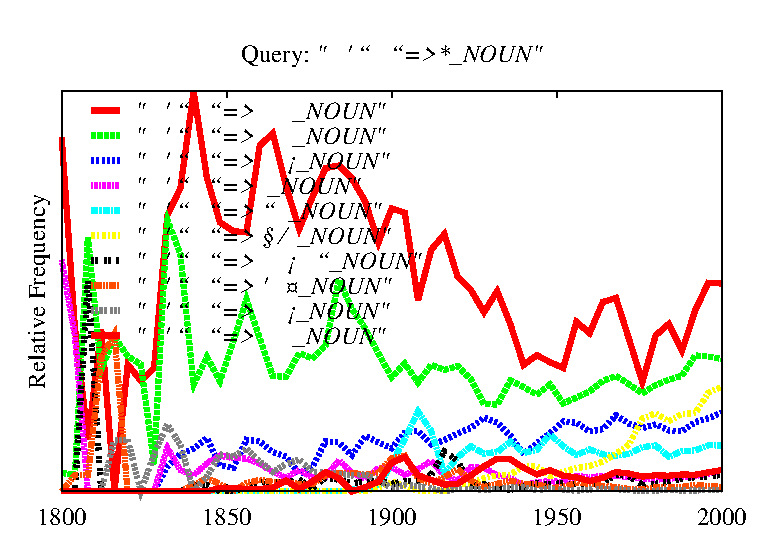
\includegraphics[width=.48\textwidth]{graphs/drink_HEB}
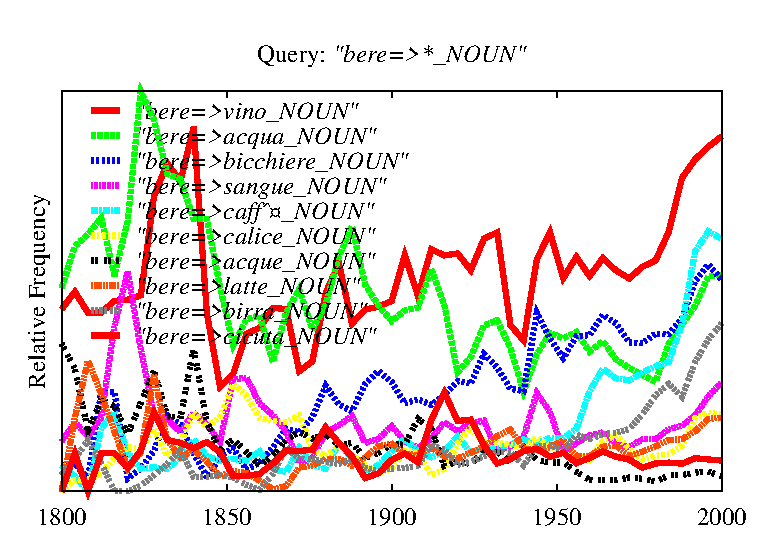
\includegraphics[width=.48\textwidth]{graphs/drink_ITA}
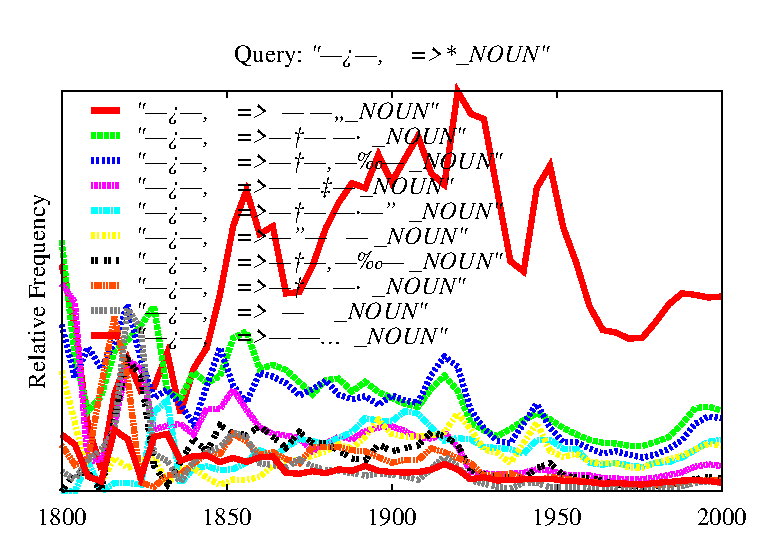
\includegraphics[width=.48\textwidth]{graphs/drink_RUS}
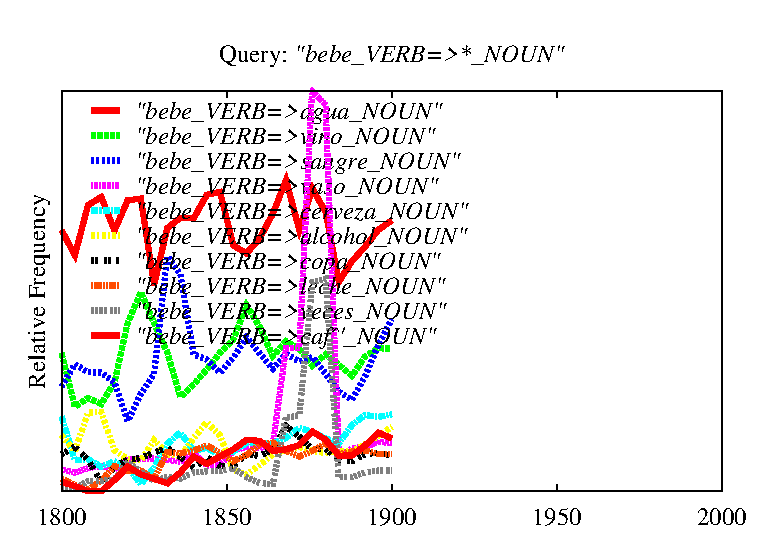
\includegraphics[width=.48\textwidth]{graphs/drink_SPA}}
\caption{\label{fig:examples}
Use Cases Highlighted}
\end{figure*}


\begin{table*}
\begin{tabular}{|l|l|l|l|l|l|l|l|l|l|}
\hline
All English                                                                                                               &  \begin{tabular}[c]{@{}c@{}}American \\English\end{tabular}                                                                                                           &  \begin{tabular}[c]{@{}c@{}}British \\English\end{tabular}                                                                                                            & German                                                                                                                                       & French                                                                                                                     & Russian                                                                                                            & Italian                                                                                                                                     & \begin{tabular}[c]{@{}c@{}}Chinese \\ (Simplified)\end{tabular}                                        & Spanish                                                                                                                            & Hebrew                                                                                                      \\ \hline \hline
\begin{tabular}[c]{@{}c@{}}water,\\ wine,\\ blood,\\ tea,\\ cup,\\ health,\\ glass,\\ beer,\\ milk,\\ coffee\end{tabular} & 
\begin{tabular}[c]{@{}c@{}}wine,\\ water,\\ cup,\\ blood,\\ tea,\\ health,\\ glass,\\ beer,\\ coffee,\\ milk,\end{tabular} & 
\begin{tabular}[c]{@{}c@{}}wine,\\ water,\\ health,\\ tea,\\ blood,\\ cup,\\ glass,\\ beer,\\ waters,\\ milk,\end{tabular} & 
\begin{tabular}[c]{@{}c@{}}Wein, \\ Glas, \\ Wasser, \\ \\ Kaffee, \\ Bier, \\ Komm, \\ Trink, \\ Schluck, \\ Milch, \\ Schnaps\end{tabular} & \begin{tabular}[c]{@{}c@{}}vin, \\ verre, \\ au, \\ sang, \\ lait, \\ coup, \\ caf�, \\ h�, \\ calice, \\ aux\end{tabular} & 
\begin{tabular}[c]{@{}c@{}}???, \\ ????, \\ ????, \\ ???, \\ ?????, \\ ????, \\ ????, \\ ????, \\????, \\ ???\end{tabular} & 
\begin{tabular}[c]{@{}c@{}}vino, \\ acqua, \\ icchiere, \\ sangue, \\ caff�, \\ calice, \\ acque, \\ latte, \\ irra, \\ cicuta\end{tabular} & 
\begin{tabular}[c]{@{}c@{}}?, \\ ?, \\ ?, \\ ??, \\ ?, \\ ??, \\ ??, \\ ??, \\ ?, \\ ?\end{tabular} & 
\begin{tabular}[c]{@{}c@{}}agua, \\ vino, \\ �, \\ sangre, \\ aguas, \\ vaso, \\ cicuta, \\ mas, \\ leche, \\ copa\end{tabular} & 
\begin{tabular}[c]{@{}c@{}}???\\ ??? \\ ???\\ ? \\ ??\\ ??? \\ ????? \\ ??? \\ ???\\ ???\end{tabular} \\ \hline
\end{tabular}
\end{table*}

\jmcomment{Automatic viewing of irregular vs regular verbs}




\section{Conclusions}
We have presented a new version of the Ngram Viewer with some new functionality. With the introduction of these new features, users can perform more powerful searches that show trends which were not possible to extract from earlier versions of the tool. The new features have been highlighted in a recent article by the Atlantic, as well on various blogs.

\jmcomment{We can cite examples from the media where this has been mentioned, and also show examples from several blog posts/entries from the internet:
http://sciencerefinery.com/2013/10/28/google-ngram-viewer-now-more-powerful-than-ever/
http://www.devingriffiths.com/google-books/google-n-gram-studies/
http://languagelog.ldc.upenn.edu/nll/?p=8472
http://www.textualscholarship.nl/?p=14051}



\bibliographystyle{acl}
\bibliography{acl2014}
\end{document}